\documentclass[12pt,letterpaper]{article}
\usepackage{graphicx,textcomp}
\usepackage{natbib}
\usepackage{setspace}
\usepackage{fullpage}
\usepackage{color}
\usepackage[reqno]{amsmath}
\usepackage{amsthm}
\usepackage{fancyvrb}
\usepackage{amssymb,enumerate}
\usepackage[all]{xy}
\usepackage{endnotes}
\usepackage{lscape}
\newtheorem{com}{Comment}
\usepackage{float}
\usepackage{hyperref}
\newtheorem{lem} {Lemma}
\newtheorem{prop}{Proposition}
\newtheorem{thm}{Theorem}
\newtheorem{defn}{Definition}
\newtheorem{cor}{Corollary}
\newtheorem{obs}{Observation}
\usepackage[compact]{titlesec}
\usepackage{dcolumn}
\usepackage{tikz}
\usetikzlibrary{arrows}
\usepackage{multirow}
\usepackage{xcolor}
\newcolumntype{.}{D{.}{.}{-1}}
\newcolumntype{d}[1]{D{.}{.}{#1}}
\definecolor{light-gray}{gray}{0.65}
\usepackage{url}
\usepackage{listings}
\usepackage{color}
\usepackage{adjustbox}

\definecolor{codegreen}{rgb}{0,0.6,0}
\definecolor{codegray}{rgb}{0.5,0.5,0.5}
\definecolor{codepurple}{rgb}{0.58,0,0.82}
\definecolor{backcolour}{rgb}{0.95,0.95,0.92}

\lstdefinestyle{mystyle}{
	backgroundcolor=\color{backcolour},   
	commentstyle=\color{codegreen},
	keywordstyle=\color{magenta},
	numberstyle=\tiny\color{codegray},
	stringstyle=\color{codepurple},
	basicstyle=\footnotesize,
	breakatwhitespace=false,         
	breaklines=true,                 
	captionpos=b,                    
	keepspaces=true,                 
	numbers=left,                    
	numbersep=5pt,                  
	showspaces=false,                
	showstringspaces=false,
	showtabs=false,                  
	tabsize=2
}
\lstset{style=mystyle}
\newcommand{\Sref}[1]{Section~\ref{#1}}
\newtheorem{hyp}{Hypothesis}

\title{Stats week 6 - Group Project}
\date{October 19, 2021}
\author{Applied Stats: Samanta, Ariana, Melisa, Felipe, Brendan}

\begin{document}
	\maketitle
	
	\section*{How to Win Awards}

	
	The client: Warner Bros. Film Studio
	The problem: Warner Bros. and their subsidiaries are having trouble winning best picture awards for their films. They want to know why that is - what do other studios have that they don't? What's different about their films? What can they do to maximise their chances of winning a best picture award?
	The task: Working in teams, you have 90 minutes to analyse the movies.csv dataset to provide insight for Warner Bros. into what makes an award-winning film. How you do that is up to your team, but you'll want to:
	\item a) Spend five or ten minutes thinking about the problem, and how you will address it as a team.
	
	\item b) Divide the workload appropriately between you. (Will you create smaller teams to focus on different aspects of the workflow? Will you have people focussing on technical assistance? Or visualisation? How will you coordinate activities? How will you share code/results?)
	
    \item c) Think about the different skills you have learned, and how you could apply these to the case at hand. Remember that any recommendations you make will be stronger if they are supported by the concepts of inference which you have learned.
    
	\item d) Make sure you have something completed within the deadline!

	\lstinputlisting[language=R, firstline=10, lastline=8]{movies.R}  
	
	\vspace{1cm}
\newpage

	\section*{Analysis & Conclusion} 
		\begin{itemize}
Our process: we plotted the correlation of pairs, as illustrated in the graphs below. We compared the means of the ‘yes’ and ’no’ probabilities of our outcome variables - best pic nom, best pic win, best actor win, best actress win, best director win, when paired with our predictor variables - runtime, imdb rating, imdb num votes, critic score, audience score. From these graphs, we were able to come to a conclusion whether there was a significant correlative relationship between the individual variables. Our results are reported below in a table. A ‘yes’ signals that the mean of outcome variable success (ie - winning award) was two standard deviations away from the mean of outcome variable failure (ie - not winning an award). ‘Maybe’ signals that the means were observably different, but not of the same statistical significance as a ‘yes’. 

	\vspace{1cm}

	\begin{table}[h!]
	\centering
	\begin{tabular}{c |c c c c c}
		
		
		variable & Runtime & IMDB Rating & IMDB number of votes & critic score & audience score \\
		\hline
		Best Picture win & yes & yes & yes & yes & yes \\
		Best Picture Nom & maybe & yes & yes &yes& yes \\
		best actor & maybe & no & no & no & no \\
		best actress & no & no & no & no & no\\
		best director & maybe & maybe & no & maybe & maybe
		
	\end{tabular}
\end{table}
	\vspace{1cm}
	
A significant advantage of proceeding with our analysis in this way is the fact that we were also able to observe confounding variables. We found that there is a high correlation between imbd score, critic score and audience score. Additionally, there is also a light correlation between number of imdb votes and: imdb rating, runtime, audience score.

	\begin{center}
		** Our findings were obtained by eye-balling our graphs (due to time constraints). 
	\end{center}

\item** Our findings were obtained by eye-balling our graphs (due to time constraints). 
	\vspace{1cm}

	\begin{center}
		
	 *** It is important to note that the sample size for ‘best pic win’ is quite small and so therefore, the obtained results in this analysis should be taken lightly and further analysis with a bigger sample size is needed. 
	 \end{center}
 
	\vspace{1cm}
	\begin{center}
		**** We decided to analyse all ‘award win’ variables because we believe that there may be a relationship between pics winning general awards and then winning best pic. 
		\vspace{1cm}
	\end{center}

\begin{center}

	\item 
	**** This dataset may be inacurate. For example the hurt locker won best picture but wasn't nominated. 
	
\end{center}
	\vspace{1cm}
To conclude, our explanatory variables generally appear not to explain variability in our outcome variables for best actress and best actor win. Our explanatory variables generally appear to contribute to variability in our outcome variables for best pic nom and best pic win. There is an insufficient evidence to reach a conclusion on best director win. 


So - we believe that Warner Bros. Studios may be more likely to obtain a win in the best pic category from longer running times, and by obtaining higher critic scores, higher imdb scores, imdb number votes, and audience scores. 
	
	\vspace{1cm}
	\end{itemize}

\newpage
			
\subsection*{Best Picture Nomination}

\lstinputlisting[language=R, firstline=2, lastline=4]{movies.R}  


\begin{figure}[h!]\centering
	\caption{\footnotesize Best Picture Nomination.}
	\label{fig:plot_1}
	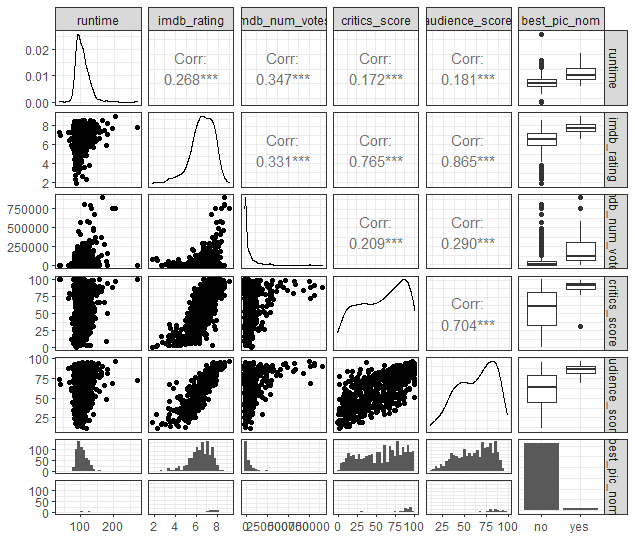
\includegraphics[width=.75\textwidth]{best pic nom 2.png}
\end{figure}

	\vspace{1cm}
	\newpage
	
\subsection*{Best Actor Win Plot}


\begin{figure}[h!]\centering
	\caption{\footnotesize Best Actor Win.}
	\label{fig:plot_2}
	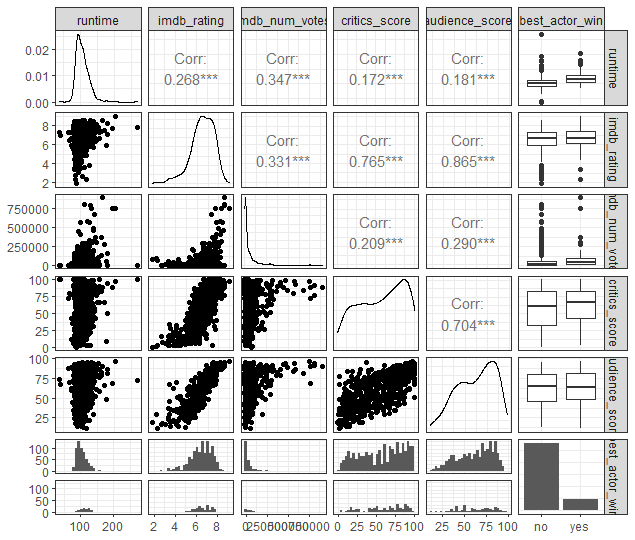
\includegraphics[width=.75\textwidth]{best actor 2.png}
\end{figure}

	\vspace{1cm}
\newpage


\subsection*{Best Actress Win Plot}

\begin{figure}[h!]\centering
	\caption{\footnotesize Best Actress Win.Plot }
	\label{fig:plot_3}
	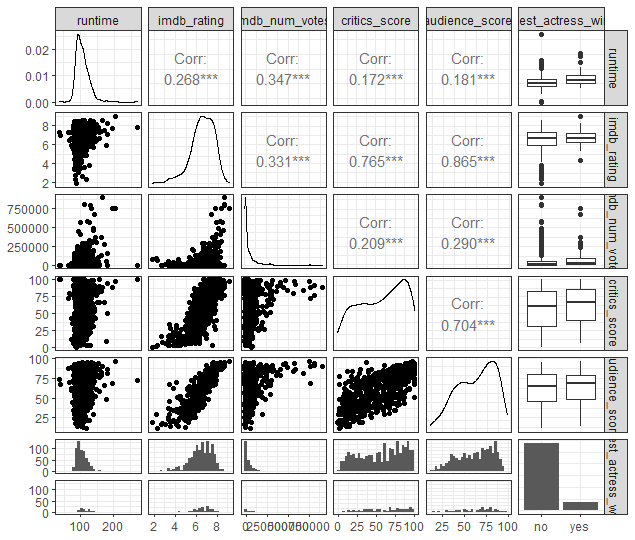
\includegraphics[width=.75\textwidth]{best actress 2.png}
\end{figure}

	\vspace{1cm}
	
	\newpage
	
\subsection*{Best Director Win}

\begin{figure}[h!]\centering
	\caption{\footnotesize Best Director Win.Plot }
	\label{fig:plot_4}
	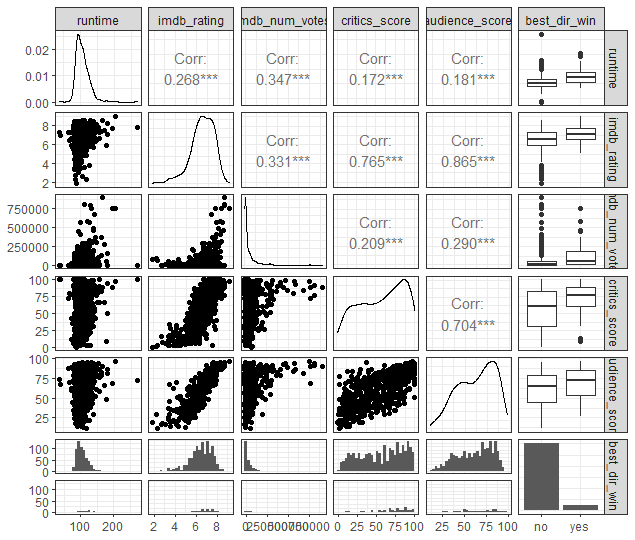
\includegraphics[width=.75\textwidth]{best dir 2.png}
\end{figure}

	\vspace{1cm}
	
	\newpage
	
\subsection*{Best Pic Win}

\lstinputlisting[language=R, firstline=42, lastline=45]{movies.R}  

\begin{figure}[h!]\centering
	\caption{\footnotesize Best Pic Win }
	\label{fig:plot_5}
	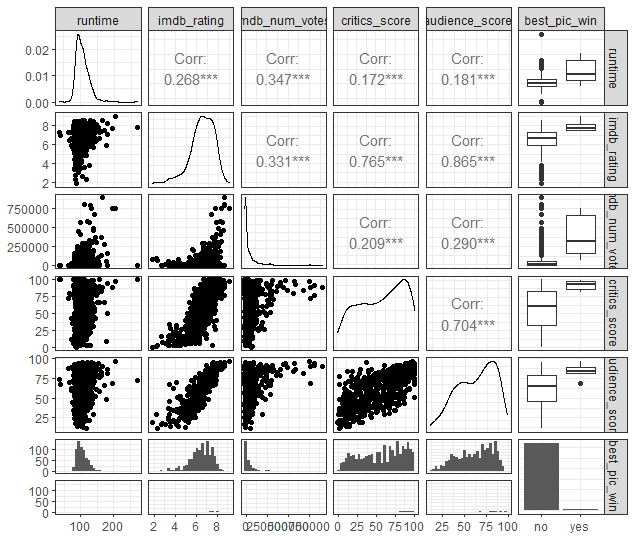
\includegraphics[width=.75\textwidth]{best pic win 2.png}
\end{figure}


	\vspace{1cm}

\end{document}
